\subsection*{Explicación}
Para este ejercicio sí use kmaps e hice una implementación vehavioral.
\subsection*{Código}
\faGithub \space
\href{https://github.com/warleon/Arch-lab1/tree/master/pregunta4}{https://github.com/warleon/Arch-lab1/tree/master/pregunta4}\\
make decimal

%\subsection*{Tabla de verdad}

\subsection*{Mapa de Karnaugh}
\begin{figure}[h]
    \centering

    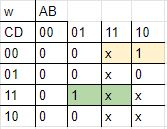
\includegraphics{fotos/kmaps/kmap1-lab1-arqui.JPG}
    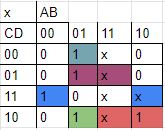
\includegraphics{fotos/kmaps/kmap2-lab1-arqui.JPG}

   
    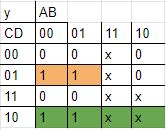
\includegraphics{fotos/kmaps/kmap3-lab1-arqui.JPG}
    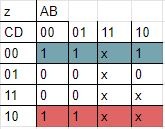
\includegraphics{fotos/kmaps/kmap4-lab1-arqui.JPG}
\end{figure}

\subsection*{Ecuaciones booleanas}
$W=A.\overline{D}+B.C.D$\\
$X=\overline{B}.C.D+B.\overline{C}.D+\overline{A}.B.\overline{D}+A.C.\overline{D}$\\
$Y=\overline{A}.\overline{C}.D+C.\overline{D}$\\
$Z=\overline{C}.\overline{D}+C.\overline{D}$\\

\subsection*{Resultados}
\begin{figure}[h]
    \centering
    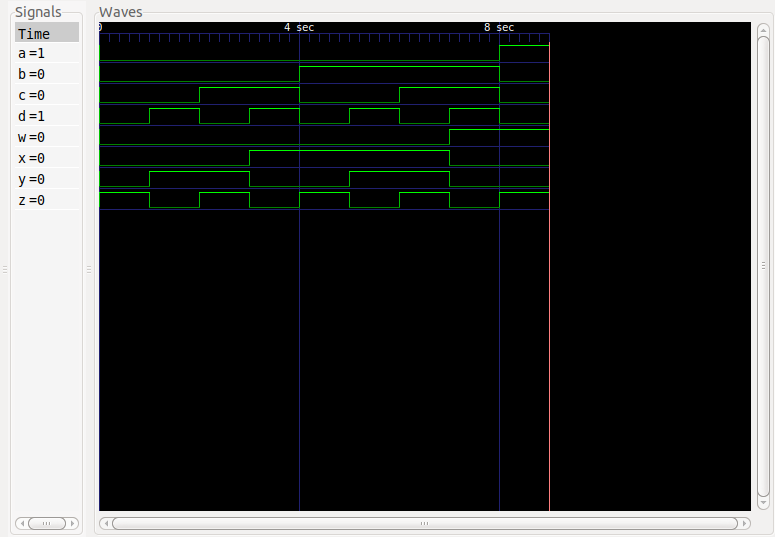
\includegraphics[scale=0.6]{fotos/resultados/arki-DECIMAL.png}
    \caption{waves BCD}
\end{figure}